%%% Local Variables:
%%% mode: latex
%%% TeX-master: "../doc"
%%% coding: utf-8
%%% End:
% !TEX TS-program = pdflatexmk
% !TEX encoding = UTF-8 Unicode
% !TEX root = ../doc.tex

Begriffe: Define AI, ML, DeepLearning, LLM\\
\cite{stoffelbauer_how_2023}\\

how llms work + popular llms

\section{LLM pipeline}

\subsection{Pre-Deployment (Training \& Preparation)}

\subsubsection{1. Base Model Pre-training}
\begin{itemize}[leftmargin=*]
    \item Train on large corpus
    \item \textbf{Data filtering/curation}: Remove toxic content, low-quality sources, copyright issues
    \item \textbf{Factual data emphasis}: Prioritize high-quality, reliable sources
    \item Some deduplication to reduce memorization
\end{itemize}

\subsubsection{2. Alignment Training }
\begin{itemize}[leftmargin=*]
    \item \textbf{RLHF (Reinforcement Learning from Human Feedback)}:
    \begin{itemize}
        \item Safety preferences (don't help with harmful requests)
        \item Helpfulness preferences
        \item \textbf{Accuracy/honesty preferences} (admit uncertainty, avoid making things up)
    \end{itemize}
    \item \textbf{Constitutional AI} or similar: Train on principles including truthfulness
    \item \textbf{Supervised fine-tuning (SFT)}:
    \begin{itemize}
        \item Curated examples of good/bad behavior
        \item Examples of admitting ``I don't know''
        \item \textbf{Calibrated uncertainty} (hedging when unsure)
    \end{itemize}
\end{itemize}

\subsubsection{3. Tool Use Training {} (for accuracy)}
\begin{itemize}[leftmargin=*]
    \item Teach model when/how to use:
    \begin{itemize}
        \item \textbf{Web search} (for current info)
        \item \textbf{Code execution} (for math/calculations)
        \item \textbf{RAG/retrieval systems} (fetch verified information)
        \item \textbf{APIs} (weather, sports scores, etc.)
    \end{itemize}
    \item Training on tool-calling patterns
\end{itemize}

\subsubsection{4. Model Optimization}
\begin{itemize}[leftmargin=*]
    \item Quantization (reduce size)
    \item Distillation (optional)
    \item Deployment optimization
\end{itemize}

\section{Inference Time (When You Use It)}

\subsubsection{5. Input Processing }
\begin{itemize}[leftmargin=*]
    \item \textbf{Safety classifiers}: Scan for harmful/inappropriate requests
    \item \textbf{Intent detection}: Understand what user is asking for
    \item \textbf{PII detection}: Flag personal information
    \item \textbf{Jailbreak detection}: Identify prompt injection attempts
    \item \textbf{Rate limiting}: Prevent abuse
\end{itemize}

\subsubsection{6. System Prompt Application }
\begin{itemize}[leftmargin=*]
    \item Instructions invisible to you (like my system prompt)
    \item Contains:
    \begin{itemize}
        \item Safety rules and guidelines
        \item \textbf{Behavioral constraints} (be helpful, honest, harmless)
        \item \textbf{Accuracy instructions} (``cite sources,'' ``admit uncertainty,'' ``use tools when needed'')
        \item \textbf{Tool usage guidance} (when to search web vs use knowledge)
        \item Knowledge cutoff date
        \item Formatting preferences
    \end{itemize}
\end{itemize}

\subsubsection{7. Context Management}
\begin{itemize}[leftmargin=*]
    \item \textbf{RAG/Retrieval {} (for factual accuracy)}
    \begin{itemize}
        \item Fetch relevant documents from knowledge base
        \item Inject verified information into context
    \end{itemize}
    \item \textbf{Tool invocation {} (hallucination prevention)}
    \begin{itemize}
        \item Trigger web search for current events
        \item Use calculators for math
        \item Fetch real-time data (weather, stocks, sports)
    \end{itemize}
    \item Conversation history management
    \item Memory systems (some models)
\end{itemize}

\subsubsection{8. Model Generation}
\begin{itemize}[leftmargin=*]
    \item Model generates response based on:
    \begin{itemize}
        \item Training (including alignment)
        \item System prompt
        \item Retrieved context
        \item User input
    \end{itemize}
\end{itemize}

\subsubsection{9. Output Processing }
\begin{itemize}[leftmargin=*]
    \item \textbf{Safety classifiers}: Scan generated output for:
    \begin{itemize}
        \item Harmful content
        \item Inappropriate responses
        \item Privacy violations (leaked training data)
    \end{itemize}
    \item \textbf{Factuality checks {} (limited)}:
    \begin{itemize}
        \item Some systems check citations exist
        \item Consistency checks
        \item \textbf{Confidence scoring} (flag low-confidence outputs)
        \item \textbf{Not very effective} -- hard to verify truth automatically
    \end{itemize}
    \item \textbf{Content filters}:
    \begin{itemize}
        \item Copyright detection (exact text matches)
        \item PII removal
    \end{itemize}
    \item Formatting adjustments
\end{itemize}

\subsubsection{10. Response Delivery}
\begin{itemize}[leftmargin=*]
    \item Show response to user
    \item \textbf{Feedback collection }
    \begin{itemize}
        \item Thumbs up/down
        \item User reports
        \item Implicit signals (regeneration requests)
    \end{itemize}
\end{itemize}

\section{Post-Deployment (Continuous Improvement)}

\subsubsection{11. Monitoring \& Logging }
\begin{itemize}[leftmargin=*]
    \item Track failure modes
    \item \textbf{Hallucination detection} (user feedback, fact-checking samples)
    \item Safety violations
    \item Usage patterns
\end{itemize}

\subsubsection{12. Feedback Loop }
\begin{itemize}[leftmargin=*]
    \item Collect user feedback
    \item \textbf{Red-teaming}: Actively try to break the model
    \item A/B testing improvements
    \item Feed back into training (next iteration)
\end{itemize}

problems with xai models

dishonesty vs hallucination

statements that contradict learned knowledge, also known as dishonesty; 2) statements that are factually incorrect and fabricated by models, that is hallucination. \cite{wu_usable_2025}

why xai is needed

xai categories

\begin{figure}
    \centering
    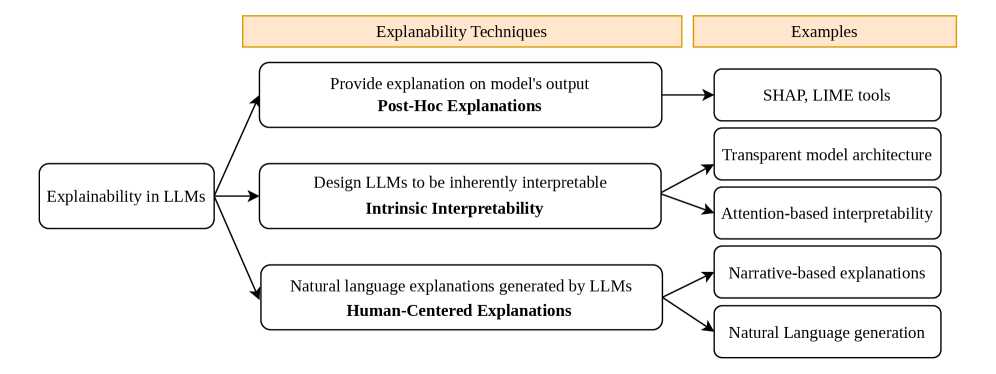
\includegraphics[width=0.9\linewidth]{img/xaicategories.png}
    \caption{XAI Categories \cite{bilal_llms_2025}}
    \label{fig:xai_categories}
\end{figure}

how xai methods work

known xai methods for llms

current mitigations: 
- Explainable Prompting Chain of Thought (CoT) / Tree of Thoughts (ToT) / Graph of Thoughts (GoT)
- Knowledge Augmented Prompting Enhancing models with external knowledge
- Training Data augmentation with explanation
- User friendly explanation with LLMs (self explanation, in context based approaches)
- interpreatable AI system design with llms

problem: no real research on what method would actually help the lay person consumer













